\documentclass[10pt,a4paper,headinclude,footinclude,hidelinks]{scrreprt} % KOMA-Script
\usepackage[italian]{babel}
\usepackage[utf8]{inputenc}
\usepackage[T1]{fontenc}
\usepackage{graphicx}
\usepackage{amsfonts}
\usepackage[]{../../classicthesis} % nochapters
\pagestyle{scrheadings}
\setcounter{tocdepth}{2}

\begin{document}
    \title{\rmfamily\normalfont\spacedallcaps{Progettazione}}
    \author{\spacedlowsmallcaps{Nicola Moretto (matr. 578258)}}
    \date{\today}
    
    \maketitle
    
    \begin{abstract}
        \noindent Il documento riporta le informazioni di progettazione riguardanti l'interfaccia grafica per la visualizzazione e la navigazione dei contenuti.
    \end{abstract}
    
	\begin{table}[ht]
	\centering
	\begin{tabular}{|c|c|l|}
	\hline
	\textsc{Versione} & \textsc{Data} & \textsc{Modifiche} \\ \hline
	0.1 & 15-10-2012 & Stesura iniziale del documento. \\ \hline
	0.2 & 17-10-2012 & Redatto il capitolo \ref{ch:stage:design:architettura}. \\ \hline
	0.3 & 18-10-2012 & Redatte le sezioni \ref{sec:stage:design:model.filter}, \ref{sec:stage:design:view.filter} e \ref{sec:stage:design:view.search}. \\ \hline
	0.4 & 19-10-2012 & Redatti i capitoli \ref{ch:stage:design:model} e \ref{ch:stage:design:view}. \\ \hline
	0.5 & 20-10-2012 & Revisione del documento. \\ \hline
	1.0 & 20-10-2012 & Pubblicazione della prima versione. \\ \hline
	1.1 & 22-10-2012 & Aggiunte la sezioni \ref{sec:stage:design:model.provider} e \ref{sec:stage:design:model.timeline}. \\ \hline
	1.2 & 23-10-2012 & Aggiornate le sezioni \ref{sec:stage:design:model.criteria} e \ref{sec:stage:design:model.filter}. \\ \hline
	1.3 & 24-10-2012 & Aggiornate le sezioni \ref{sec:stage:design:model} e \ref{sec:stage:design:model.search}. \\ \hline
	1.4 & 26-10-2012 & Aggiornato il capitolo \ref{ch:stage:design:view}. \\ \hline
	1.5 & 27-10-2012 & Aggiunti i capitoli \ref{ch:stage:design:pattern} e \ref{ch:stage:design:tracciamento}. \\ \hline
	2.0 & 28-10-2012 & Pubblicazione della seconda versione. \\ \hline
%	2.1 & 29-10-2012 & \ldots \\ \hline
	\end{tabular}
	\caption{Registro delle modifiche}
	\label{tab:stage:wp:workload}
	\end{table}

	\tableofcontents

	\listoffigures

	%----------
	% CAPITOLO
	%----------
	\chapter{Introduzione}
	\label{ch:stage:design:intro}

	\section{Convenzioni}
	La nomenclatura adottata per i package e le classi è il \textit{CamelCase}.	L'identificatore di ciascuna sottoclasse adotta come prefisso le lettere maiuscole presenti nel nome della rispettiva classe base (nel medesimo ordine di apparizione).

	\section{Riferimenti informativi}
	\begin{itemize}
	\item Analisi dei requisiti (\textit{analisi\_dei\_requisiti\_1.0} allegata alla presente documentazione);
	\item Sistema di classificazione (\textit{sistema\_di\_classificazione\_2.0} allegato alla presente documentazione).
	\end{itemize}

	%----------
	% CAPITOLO
	%----------
	\chapter{Architettura}
	\label{ch:stage:design:architettura}

	\section{Architettura generale}
	\label{sec:stage:design:architettura:mvc}
	L'architettura del sistema software rispecchia il design pattern architetturale MVC, che prevede e garantisce la separazione delle tre componenti fondamentali del sistema:
	\begin{description}
	\item[Model] Racchiude i dati e le informazioni dell'applicazione e definisce le modalità di accesso e fruizione degli stessi da parte delle altre componenti (\textit{Controller} e \textit{View}).
 	\item[View] Rappresenta l'interfaccia grafica mediante la quale vengono visualizzate le informazioni e i dati conservati nel \textit{Model} e l'utente può interagire con il sistema. La rilevazione dell'avvenuta interazione dell'utente è responsabilità di tale componente, mentre la gestione della reazione è demandata al \textit{Controller}.
	\item[Controller] Incorpora la logica di controllo dell'applicazione, inizializzando il sistema e traducendo l'interazione dell'utente con l'interfaccia grafica (\textit{View}) in operazioni sui dati (\textit{Model}).
	\end{description}

	\section{Componenti architetturali}
	\label{sec:stage:design:mvc}

	\subsection{Componente Model}
	\label{sec:stage:design:mvc:model}
	La componente \textit{model} conserva tutte i tipi di informazioni connessi alla ricerca:
	\begin{itemize}
	\item gli ambiti (etichette, frasi);
	\item i criteri (termini di ricerca, entità);
	\item i filtri (argomento, data di pubblicazione, emozioni, \ldots);
	\item i risultati (contenuti informativi).
	\end{itemize}

	\subsection{Componente View}
	\label{sec:stage:design:mvc:view}
	La componente \textit{view} rappresenta l'interfaccia grafica mediante la quale l'utente interagisce con il sistema per effettuare una ricerca, raffinarne i criteri o consultarne i risultati.

	\paragraph{Livelli}
	Essa è organizzata in quattro livelli (o strati) distinti, che includono rispettivamente:
	\begin{itemize}
	\item gli strumenti e le informazioni connesse alla ricerca (barra di ricerca, etichette, entità, \ldots);
	\item i filtri di ricerca;
	\item i risultati della ricerca (proprietà e relazioni dei contenuti informativi;
	\item la cronologia (organizzazione temporale dei contenuti).
	\end{itemize}

	\subsection{Componente Controller}
	\label{sec:stage:design:mvc:controller}
	La componente \textit{controller} gestisce l'interazione dell'utente con l'interfaccia grafica e le operazioni connesse alla ricerca e alla visualizzazione dei contenuti informativi, tra cui:
	\begin{itemize}
	\item la configurazione dei criteri di ricerca (selezione di un'accezione di un'etichetta, gestione delle entità);
	\item il reperimento dei contenuti informativi corrispondenti ai criteri di ricerca;
	\item la gestione dei filtri di ricerca;
	\item l'aggiornamento dei risultati di ricerca visualizzati a fronte di modifiche alle entità e ai filtri di ricerca;
	\item \ldots
	\end{itemize}

	%----------
	% CAPITOLO
	%----------
	\chapter{Componente Model}
	\label{ch:stage:design:model}

	\begin{figure}[ht]
		\begin{center}
	    	\includegraphics[width=10cm]{package/model.png}
			\label{gfx:package:model}
			\caption{Diagramma del package \textit{model}}
		\end{center}
	\end{figure}

	Questo capitolo illustra i componenti del \textit{Model}, per ciascuno dei quali è indicato il nome della classe accompagnata da un'identificazione sintetica, separati dal carattere '|' (separatore verticale).

	% SECTION
	\section{Package model}
	\label{sec:stage:design:model}

	\begin{figure}[ht]
		\begin{center}
	    	\includegraphics[width=10cm]{class/model.png}
			\label{gfx:package:model:model}
			\caption{Diagramma delle classi del package \textit{model}}
		\end{center}
	\end{figure}

	\subsection[Content]{Content | Contenuto informativo}
	\label{sec:stage:design:model:content}
	La classe rappresenta un generico contenuto informativo pubblicato dagli utenti nella piattaforma, caratterizzato dalle seguenti proprietà:
	\begin{itemize}
	\item autore (\textit{\nameref{sec:stage:design:model.criteria:user}});
	\item data di pubblicazione (\textit{\nameref{sec:stage:design:model.criteria:publication-date}});
	\item titolo.
	\end{itemize}

	A ciascun contenuto sono inoltre associate informazioni aggiuntive di classificazione:
	\begin{itemize}
	\item argomento (\textit{\nameref{sec:stage:design:model.criteria:topic}});
	\item emozioni (\textit{\nameref{sec:stage:design:model.criteria:emotion}});
	\item giudizio (\textit{\nameref{sec:stage:design:model.criteria:rating}});
	\item entità (\textit{\nameref{sec:stage:design:model:entity}});
	\item intenzioni (\textit{\nameref{sec:stage:design:model.criteria:intention}});
	\item interessi (\textit{\nameref{sec:stage:design:model.criteria:interest}}).
	\end{itemize}

	\subsection[CAnswer]{CAnswer | Risposta}
	\label{sec:stage:design:model:answer}
	La classe rappresenta un contenuto di tipo \textit{risposta} ed estende la classe \textit{\nameref{sec:stage:design:model:content}}.

	\subsection[CEvent]{CEvent | Evento}
	\label{sec:stage:design:model:event}
	La classe rappresenta un contenuto di tipo \textit{evento} ed estende la classe \textit{\nameref{sec:stage:design:model:content}}.

	\subsection[CMessage]{CMessage | Comunicazione privata}
	\label{sec:stage:design:model:message}
	La classe rappresenta un contenuto di tipo \textit{comunicazione privata} ed estende la classe \textit{\nameref{sec:stage:design:model:content}}.

	\subsection[CQuestion]{CQuestion | Domanda}
	\label{sec:stage:design:model:question}
	La classe rappresenta un contenuto di tipo \textit{domanda} ed estende la classe \textit{\nameref{sec:stage:design:model:content}}.

	\subsection[CReview]{CReview | Recensione}
	\label{sec:stage:design:model:review}
	La classe rappresenta un contenuto di tipo \textit{recensione} ed estende la classe \textit{\nameref{sec:stage:design:model:content}}.

	\subsection[CTalk]{CTalk | Discorso}
	\label{sec:stage:design:model:talk}
	La classe rappresenta un contenuto di tipo \textit{discorso} ed estende la classe \textit{\nameref{sec:stage:design:model:content}}.

	\subsection[CThought]{CThought | Pensiero}
	\label{sec:stage:design:model:thought}
	La classe rappresenta un contenuto di tipo \textit{pensiero} ed estende la classe \textit{\nameref{sec:stage:design:model:content}}.

	\subsection[Entity]{Entity | Entità del dominio}
	\label{sec:stage:design:model:entity}
	La classe modella un'entità del dominio della piattaforma, cui è associata un'etichetta - in una specifica accezione - che la identifica univocamente nell'ambito della piattaforma (\textit{\nameref{sec:stage:design:model:label}}).

	\subsection[EntityType]{EntityType | Tipo di entità}
	\label{sec:stage:design:model:entity-type}
	La classe rappresenta i tipi delle entità (\textit{\nameref{sec:stage:design:model:entity}}).

	\subsection[Label]{Label | Etichetta del dizionario}
	\label{sec:stage:design:model:label}
	La classe modella le etichette del dizionario della piattaforma, ciascuna delle quali può possedere molteplici accezioni (\textit{\nameref{sec:stage:design:model:meaning}}).

	\subsection[Meaning]{Meaning | Accezione di un'etichetta}
	\label{sec:stage:design:model:meaning}
	La classe modella un'accezione di un'etichetta (\textit{\nameref{sec:stage:design:model:label}}), che riferisce un'entità del dominio (\textit{\nameref{sec:stage:design:model:entity}}).

	% SECTION
	\section{Package model.criteria}
	\label{sec:stage:design:model.criteria}
	Ciascun contenuto può essere classificato in accordo a differenti criteri, ciascuno dei quali ne prende in esame una proprietà (autore, data di pubblicazione, tipo), un criterio di classificazione (emozioni, intenzioni, \ldots) o un informazione contestuale alla ricerca (attinenza, \ldots) differenti.

	\subsection[CriterionModel]{CriterionModel | Gestione dei criteri di classificazione}
	\label{sec:stage:design:model.criteria:criteria-model}
	La classe \textit{\nameref{sec:stage:design:model.criteria:criteria-model}} rappresenta l'interfaccia del package \textit{model.criteria}.

	\subsection[CriterionType]{CriterionType | Classe dei criteri di classificazione}
	\label{sec:stage:design:model.criteria:criteria}
	Tale componente rappresenta un'interfaccia per le classi dei criteri di classificazione.

	\subsection[CTList]{CTList | Criterio basato su una lista di valori}
	\label{sec:stage:design:model.criteria:list-criterion}
	La classe \textit{\nameref{sec:stage:design:model.criteria:list-criterion}} rappresenta un criterio di classificazione basato su una lista di valori, ciascuno dei quali può essere ammissibile o bloccato. Ciascuna istanza viene utilizzata in combinazione con un filtro \textit{\nameref{sec:stage:design:model.filter:list-filter}}, fornendo i valori e i parametri di configurazione iniziale.

	\subsection[CTRange]{CTRange | Criterio basati su un intervallo di valori}
	\label{sec:stage:design:model.criteria:range-criterion}
	La classe \textit{\nameref{sec:stage:design:model.criteria:range-criterion}} rappresenta un criterio di classificazione basato su un intervallo di valori. Ciascuna istanza viene utilizzata in combinazione con un filtro \textit{\nameref{sec:stage:design:model.filter:range-filter}}, fornendo i valori e i parametri di configurazione iniziale.

	\subsection[CTSwitch]{CTSwitch | Criterio a doppio stato}
	\label{sec:stage:design:model.criteria:switch-criterion}
	La classe \textit{\nameref{sec:stage:design:model.criteria:switch-criterion}} rappresenta un criterio di classificazione che l'utente può semplicemente decidere di attivare o disattivare. Ciascuna istanza viene utilizzata in combinazione con un filtro \textit{\nameref{sec:stage:design:model.filter:switch-filter}}, fornendo i valori e i parametri di configurazione iniziale.

	\subsection[CTValue]{CTValue | Filtro basato su una soglia di valore}
	\label{sec:stage:design:model.criteria:value-criterion}
	La classe \textit{\nameref{sec:stage:design:model.criteria:value-criterion}} rappresenta un criterio di classificazione basato su una soglia di valore. Ciascuna istanza viene utilizzata in combinazione con un filtro \textit{\nameref{sec:stage:design:model.filter:value-filter}}, fornendo i valori e i parametri di configurazione iniziale.

	\subsection[CriterionData]{CriterionData | Sorgente dati per un criterio di classificazione}
	\label{sec:stage:design:model.criteria:criterion-data}
	La classe astratta \textit{\nameref{sec:stage:design:model.criteria:criterion-data}} incapsula le informazioni (parametri di configurazione, valori, \ldots) necessari ad inizializzare un oggetto di tipo \textit{\nameref{sec:stage:design:model.criteria:criteria}}.
	% Campo dati statico: riferimento ai risultati di ricerca
	% Sottoclassi: metodo statico che restituisce i valori richiesti (lista, min, max, ...)
	% Sottoclasse lista con valori predefiniti: campo dati statico con lista di valori dello stesso tipo della classe

	\subsection[CDEmotion]{CDEmotion | Emozione}
	\label{sec:stage:design:model.criteria:emotion}
	La classe rappresenta un'emozione associabile ad un contenuto e ne fornisce la lista completa. Le relative istanze vengono impiegate in combinazione con oggetti di tipo \textit{\nameref{sec:stage:design:model.criteria:list-criterion}}.

	\subsection[CDIntention]{CDIntention | Intenzione}
	\label{sec:stage:design:model.criteria:intention}
	La classe rappresenta un'intenzione associata ad un contenuto e ne fornisce la lista completa. Le relative istanze vengono impiegate in combinazione con oggetti di tipo \textit{\nameref{sec:stage:design:model.criteria:list-criterion}}.

	\subsection[CDInterest]{CDInterest | Interessi dell'utente}
	\label{sec:stage:design:model.criteria:interest}
	La classe fornisce la lista degli interessi scelti da un utente (\textit{\nameref{sec:stage:design:model.criteria:user}}) e ciascuna istanza viene impiegata in combinazione con oggetti di tipo \textit{\nameref{sec:stage:design:model.criteria:switch-criterion}}.

	\subsection[CDPublicationDate]{CDPublicationDate | Data di pubblicazione}
	\label{sec:stage:design:model.criteria:publication-date}
	La classe rappresenta una generica data di pubblicazione di un contenuto e fornisce la data minima e massima di pubblicazione di quelli corrispondenti ai criteri di ricerca (\textit{\nameref{sec:stage:design:model.search:search-result}}) e l'unità temporale predefinita.

	Ciascuna istanza viene impiegata in combinazione con oggetti di tipo \textit{\nameref{sec:stage:design:model.criteria:range-criterion}}.

	\subsection[CDRating]{CDRating | Giudizio}
	\label{sec:stage:design:model.criteria:rating}
	La classe rappresenta il giudizio assegnato ad un contenuto e fornisce il giudizio minimo e massimo assegnabile ad un contenuto. Ciascuna istanza viene impiegata in combinazione con oggetti di tipo \textit{\nameref{sec:stage:design:model.criteria:value-criterion}}.

	\subsection[CDRelevance]{CDRelevance | Attinenza}
	\label{sec:stage:design:model.criteria:relevance}
	La classe fornisce il grado di attinenza minimo e massimo di un contenuto rispetto ai criteri di ricerca e ciascuna istanza viene impiegata in combinazione con oggetti di tipo \textit{\nameref{sec:stage:design:model.criteria:value-criterion}}.

	\subsection[CDTopic]{CDTopic | Argomento}
	\label{sec:stage:design:model.criteria:topic}
	La classe rappresenta un generico argomento cui può appartenere un contenuto e ne fornisce la lista completa. Le relative istanze vengono impiegate in combinazione con oggetti di tipo \textit{\nameref{sec:stage:design:model.criteria:list-criterion}}.

	\subsection[CDType]{CDType | Tipo di contenuto}
	\label{sec:stage:design:model.criteria:type}
	La classe rappresenta un tipo di contenuto e ne fornisce la lista completa. Ciascuna istanza viene impiegata in combinazione con oggetti di tipo \textit{\nameref{sec:stage:design:model.criteria:list-criterion}}.

	\subsection[CDUser]{CDUser | Utente}
	\label{sec:stage:design:model.criteria:user}
	La classe rappresenta un utente della piattaforma e le relative istanze vengono impiegate in combinazione con oggetti di tipo \textit{\nameref{sec:stage:design:model.criteria:list-criterion}}.

	% SECTION	
	\section{Package model.filter}
	\label{sec:stage:design:model.filter}
	Ciascun filtro è associato ad un possibile criterio di classificazione (\textit{\nameref{sec:stage:design:model.criteria:criteria}}) e partiziona automaticamente l'insieme dei possibili valori (\textit{\nameref{sec:stage:design:model.criteria:criterion-data}}) in due sottoinsiemi: ammessi o bloccati.

	Nella configurazione iniziale, tutti i valori possibili di una proprietà sono ammessi, mentre l'utente può intervenire secondo modalità differenti per alterare tale partizionamento (vedi sezione \ref{sec:stage:design:view.filter}).
	
	Il valore che ciascun contenuto (risultato di una ricerca) assume in relazione ad una proprietà associata ad un filtro può quindi appartenere ad uno dei due sottoinsiemi: il contenuto viene mostrato solo se tutti i valori delle proprietà in questione risultano ammessi.

	\subsection[FilterFactory]{FilterFactory | Creazione dei filtri}
	\label{sec:stage:design:model.filter:filter-factory}
	La classe \textit{\nameref{sec:stage:design:model.filter:filter-factory}} offre un'interfaccia per creare filtri (\textit{\nameref{sec:stage:design:model.filter:filter}}) basati sui possibili criteri (\textit{\nameref{sec:stage:design:model.criteria:criterion-data}}) in modo trasparente rispetto al client. 

	\subsection[FilterModel]{FilterModel | Gestione dei filtri}
	\label{sec:stage:design:model.filter:filter-manager}
	Tale componente rappresenta l'interfaccia del package \textit{model.filter}, utile a esporre le funzionalità per l'istanziazione e la gestione dei filtri.

	\subsection[FilterType]{FilterType | Filtro di ricerca}
	\label{sec:stage:design:model.filter:filter}
	Tale componente rappresenta l'interfaccia dei filtri per il raffinamento dei risultati di una ricerca e viene implementata dalle classi che modellano le tipologie standard di filtri di ricerca (\textit{\nameref{sec:stage:design:model.filter:list-filter}}, \textit{\nameref{sec:stage:design:model.filter:range-filter}}, \textit{\nameref{sec:stage:design:model.filter:switch-filter}} e \textit{\nameref{sec:stage:design:model.filter:value-filter}}).
	
	Ciascuna istanza di una sottoclasse concreta è associata ai risultati di una ricerca specifica (\textit{\nameref{sec:stage:design:model.search:search-result}}), su cui si applica il filtro corrispondente.

	\subsection[FTList]{FTList | Filtro a lista di valori}
	\label{sec:stage:design:model.filter:list-filter}
	La classe \textit{\nameref{sec:stage:design:model.filter:list-filter}} modella un filtro basato su una lista di possibili valori, ciascuno dei quali può essere autorizzato o bloccato dall'utente, e ciascuna delle relative istanze è associata ad un criterio \textit{\nameref{sec:stage:design:model.criteria:list-criterion}}.

	\subsection[FTRange]{FTRange | Filtro ad intervallo di valori}
	\label{sec:stage:design:model.filter:range-filter}
	La classe \textit{\nameref{sec:stage:design:model.filter:range-filter}} modella un filtro basato su un intervallo di valori ordinati (numeri, date, \ldots) e ciascuna istanza è associata ad un criterio \textit{\nameref{sec:stage:design:model.criteria:range-criterion}}.

	Siano $inf$ e $sup$ rispettivamente l'estremo inferiore e superiore dell'intervallo: risultano dunque ammessi tutti e soli i valori $v$ tali che $v \in \left[inf,sup\right]$.

	All'utente è consentito scegliere i valori desiderati di $inf$ e $sup$ tali che:
	\begin{itemize}
	\item $sup$ e $inf$ siano valori validi;
	\item $inf \leq sup$;
	\item se è definito un valore attuale $current$, allora deve valere $min \leq current \leq max$.
	\end{itemize}

	Se l'insieme dei valori ordinati prevede un minimo $min$ e/o un massimo $max$ si aggiungono le seguenti condizioni:
	\begin{itemize}
	\item $sup \leq max$;
	\item $inf \geq min$.
	\end{itemize}

	\subsection[FTSwitch]{FTSwitch | Filtro a doppio stato}
	\label{sec:stage:design:model.filter:switch-filter}
	La classe \textit{\nameref{sec:stage:design:model.filter:switch-filter}} modella un filtro il cui partizionamento è predefinito e invariabile e che l'utente può solamente abilitare o disattivare. Ciascuna istanza è associata ad un criterio \textit{\nameref{sec:stage:design:model.criteria:switch-criterion}}.

	\subsection[FTValue]{FTValue | Filtro a soglia di valore}
	\label{sec:stage:design:model.filter:value-filter}
	La classe \textit{\nameref{sec:stage:design:model.filter:value-filter}} rappresenta un filtro basato su una soglia di valore, ciascuna delle cui istanze è associata ad un criterio \textit{\nameref{sec:stage:design:model.criteria:value-criterion}}.

	Sia $value$ il valore scelto: in tal caso risultano ammessi tutti e soli i valori $x$ validi tali che $x \geq value$. Se l'insieme prevede un minimo $min$ e/o un massimo $max$ dev'essere soddisfatta anche la condizione $min \leq x \leq max$.

	% SECTION	
	\section{Package model.provider}
	\label{sec:stage:design:model.provider}

	\begin{figure}[ht]
		\begin{center}
	    	\includegraphics[height=8cm]{class/model_provider.png}
			\label{gfx:package:model:provider}
			\caption{Diagramma delle classi del package \textit{model.provider}}
		\end{center}
	\end{figure}

	Le classi del package \textit{model.provider} forniscono un livello di astrazione per accedere alla base di dati e interrogarla al fine di reperire i contenuti informativi corrispondenti ai criteri di ricerca immessi e all'ambito specificato.

	Dal momento che tali operazioni verranno affidate a componenti terze, tuttora oggetto di analisi e valutazione, le scelte progettuali illustrate di seguito cercano di tenere conto di tale incertezza.

	\subsection[Provider]{Provider | Motore di ricerca}
	\label{sec:stage:design:model.search:search-provider}
	La componente rappresenta l'interfaccia standard implementata dai fornitori di ricerca (\textit{\nameref{sec:stage:design:model.search:tag-provider}}, \textit{\nameref{sec:stage:design:model.search:full-text-provider}}).

	\subsection[ProviderModel]{ProviderModel | Gestore motori di ricerca}
	\label{sec:stage:design:model.search:provider-model}
	La classe \textit{\nameref{sec:stage:design:model.search:provider-model}} rappresenta l'interfaccia del package \textit{model.provider} e fornisce i metodi per accedere alle funzionalità di ricerca.

	\subsection[ProviderRegistry]{ProviderRegistry | Gestione dei fornitori di ricerca}
	\label{sec:stage:design:model.search:provider-registry}
	La classe \textit{\nameref{sec:stage:design:model.search:provider-registry}} gestisce gli oggetti di tipo \textit{\nameref{sec:stage:design:model.search:search-provider}}.

	\subsection[PLabel]{PLabel | Ricerca delle etichette}
	\label{sec:stage:design:model.search:tag-provider}
	La classe \textit{\nameref{sec:stage:design:model.search:tag-provider}} fornisce le funzionalità necessaria a cercare i termini di ricerca tra le etichette assegnate ai contenuti, considerandone le specifiche accezioni.

	Essa implementa l'interfaccia \textit{\nameref{sec:stage:design:model.search:search-provider}} e le sue istanze vengono gestite da \textit{\nameref{sec:stage:design:model.search:provider-registry}}.

	\subsection[PFullText]{PFullText | Ricerca dei contenuti informativi}
	\label{sec:stage:design:model.search:full-text-provider}
	La classe \textit{\nameref{sec:stage:design:model.search:full-text-provider}} permette di cercare la presenza dei termini di ricerca nel titolo, nel corpo o in altri campi di un contenuto informativo.

	Essa implementa l'interfaccia \textit{\nameref{sec:stage:design:model.search:search-provider}} e le sue istanze vengono gestite da \textit{\nameref{sec:stage:design:model.search:provider-registry}}.

	% SECTION	
	\section{Package model.search}
	\label{sec:stage:design:model.search}
	Il package \textit{model.search} raccoglie e gestisce le informazioni inerenti i parametri e i risultati di una ricerca. 

	\subsection[Search]{Search | Gestione della ricerca}
	\label{sec:stage:design:model.search:search}
	Tale componente rappresenta l'interfaccia del package \textit{model.search}.

	\subsection[EntityList]{EntityList | Lista delle entità cercate}
	\label{sec:stage:design:model.search:search-entity-list}
	La classe \textit{\nameref{sec:stage:design:model.search:search-entity-list}} rappresenta la lista delle entità individuate a partire dai termini di ricerca corrispondenti ad etichette del dizionario.

	\subsection[Query]{Query | Query di ricerca}
	\label{sec:stage:design:model.search:search-query}
	La classe \textit{\nameref{sec:stage:design:model.search:search-query}} rappresenta la query di ricerca, ossia la stringa inserita dall'utente nella barra di ricerca (\textit{\nameref{sec:stage:design:view.search:search-bar}}) e contenente una lista di termini o espressioni separati da virgola.

	La classe fornisce i metodi per effettuare l'analisi sintattica della stringa al fine di estrapolare i termini (\textit{\nameref{sec:stage:design:model.search:search-term}}) da cercare e stabilire quali di essi siano etichette o frasi.

	\subsection[Result]{Result | Risultati della ricerca}
	\label{sec:stage:design:model.search:search-result}
	La classe \textit{\nameref{sec:stage:design:model.search:search-result}} rappresenta l'insieme dei risultati di una ricerca (\textit{\nameref{sec:stage:design:model:content}}).

	\subsection[Scope]{Scope | Ambito di ricerca}
	\label{sec:stage:design:model.search:search-scope}
	La classe \textit{\nameref{sec:stage:design:model.search:search-scope}} rappresenta un ambito di ricerca e ne rende disponibile la lista completa.

	\subsection[Term]{Term | Termine di ricerca}
	\label{sec:stage:design:model.search:search-term}
	La classe \textit{\nameref{sec:stage:design:model.search:search-term}} rappresenta un generico termine di ricerca, estrapolato dalla query (\textit{\nameref{sec:stage:design:model.search:search-query}}).

	% SECTION	
	\section{Package model.timeline}
	\label{sec:stage:design:model.timeline}
	Il package \textit{model.timeline} raccoglie le informazioni inerenti l'organizzazione e la visualizzazione cronologica dei contenuti.

	\subsection[Timeline]{Timeline | Linea del tempo}
	\label{sec:stage:design:model.timeline:timeline}
	La classe \textit{\nameref{sec:stage:design:model.timeline:timeline}} rappresenta la linea del tempo, suddivisa in intervalli temporali \textit{\nameref{sec:stage:design:model.timeline:time-unit}} di ampiezza fissa - personalizzabile dall'utente - in cui vengono collocati i risultati della ricerca o i contenuti di una discussione.

	\subsection[TimeUnit]{TimeUnit | Unità temporale}
	\label{sec:stage:design:model.timeline:time-unit}
	La classe \textit{\nameref{sec:stage:design:model.timeline:time-unit}} rappresenta un singolo intervallo di tempo e raccoglie i risultati di ricerca o i contenuti di una discussione pubblicati nel periodo corrispondente.

	%----------
	% CAPITOLO
	%----------
	\chapter{Componente View}
	\label{ch:stage:design:view}

	\begin{figure}[ht]
		\begin{center}
	    	\includegraphics[width=10cm]{package/view.png}
			\label{gfx:package:view}
			\caption{Diagramma del package \textit{view}}
		\end{center}
	\end{figure}

	Questo capitolo illustra i componenti del \textit{View}, per ciascuno dei quali è indicato il nome della classe accompagnata da un'identificazione sintetica, separati dal carattere '|' (separatore verticale).

	% SECTION
	\section{Package view}
	\label{sec:stage:design:view}
	
	\subsection[MainWindow]{MainWindow | Finestra principale}
	\label{sec:stage:design:view:window}
	La classe \textit{\nameref{sec:stage:design:view:window}} rappresenta la finestra principale all'interno del quale vengono inseriti e opportunamente collocati tutti gli elementi grafici dell'interfaccia, tra cui gli strumenti di ricerca, i filtri e i contenuti.

	% SECTION
	\section{Package view.content}
	\label{sec:stage:design:view.content}

	\subsection[ContentWidget]{ContentWidget | Contenuto informativo}
	\label{sec:stage:design:view:content-widget}
	Si tratta del componente grafico deputato a rappresentare graficamente un contenuto (\textit{\nameref{sec:stage:design:model:content}}) e le relative informazioni (in formato grafico o testuale).

	\begin{figure}[ht]
		\begin{center}
	    	\includegraphics[]{mockup/contenuto.png}
			\label{gfx:mockup:content}
			\caption{Informazioni essenziali di un contenuto}
		\end{center}
	\end{figure}

	Le informazioni essenziali\marginpar{Informazioni essenziali} sono utili per una immediato e preciso inquadramento del contenuto da parte dell'utente al fine di stabilirne la rilevanza soggettiva:
	\begin{description}
	\item[Autore] L'autore del contenuto è l'utente (\textit{\nameref{sec:stage:design:model.criteria:user}}) che lo ha pubblicato all'interno della piattaforma e viene rappresentato testualmente mediante il suo \textit{nome utente} o \textit{proprio}.
	\item[Attinenza] Il grado di attinenza di un contenuto rispetto ai criteri di ricerca (\textit{\nameref{sec:stage:design:model.criteria:relevance}}) corrisponde - in percentuale - al rapporto tra le entità assegnate e quelle cercate. Tale informazione viene rappresentata graficamente variando proporzionalmente la \textit{dimensione} dell'elemento grafico.
	\item[Data di pubblicazione] La data di pubblicazione del contenuto viene indicata testualmente.
	\item[Tipo] Il tipo di contenuto (\textit{\nameref{sec:stage:design:model.criteria:type}}) viene rappresentato graficamente variando la forma\footnote{Le forme utilizzate sono elementari per garantire l'immediata riconoscibilità da parte di qualsiasi tipo di utente, evitando l'impiego di forme potenzialmente ambigue o ignote a seconda del suo profilo sociale, culturale, geografico, \ldots} dell'elemento grafico.
	\item[Titolo] Il titolo assegnato al contenuto viene rappresentata in formato testuale.
	\end{description}

	\begin{figure}[ht]
		\begin{center}
	    	\includegraphics[]{mockup/dettagli_contenuto.png}
			\label{gfx:mockup:content-details}
			\caption{Informazioni aggiuntive di un contenuto}
		\end{center}
	\end{figure}

	Le informazioni aggiuntive\marginpar{informazioni aggiuntive} forniscono all'utente dettagli utili per approfondire l'esame di un contenuto.
	\begin{description}
	\item[Argomento] Ciascun contenuto può riferirsi al più ad un argomento (\textit{\nameref{sec:stage:design:model.criteria:topic}}), rappresentabile in maniera grafica (colore o simbolo) o testuale.
	\item[Emozioni] A ciascun contenuto possono essere associate diverse emozioni (\textit{\nameref{sec:stage:design:model.criteria:emotion}}), che esprimono lo stato d'animo dell'autore al momento della sua redazione o pubblicazione. La lista delle emozioni associate ad un contenuto viene visualizzata in formato testuale.
	\item[Entit\`a] A ciascun contenuto possono essere assegnate delle etichette (\textit{\nameref{sec:stage:design:model:label}}), che riferiscono altrettante entità del dominio da visualizzare in formato testuale (mediante il rispettivo nome).
	\item[Giudizio] Il giudizio ((\textit{\nameref{sec:stage:design:model.criteria:rating}})) associato ad un contenuto è un'informazione rappresentabile in formato testuale o grafico.
	\item[Intenzioni] A ciascun contenuto possono essere associate delle intenzioni (\textit{\nameref{sec:stage:design:model.criteria:intention}}), che possano fornire delle linee guida interpretative ai lettori. La lista delle intenzioni associate ad un contenuto viene visualizzata in formato testuale.
	\end{description}

	\subsection[EntityWidget]{EntityWidget | Contenuto informativo}
	\label{sec:stage:design:view:entity-widget}
	La classe \textit{\nameref{sec:stage:design:view:entity-widget}} rappresenta il componente grafico deputato a visualizzare le informazioni essenziali associate ad un'entità e a consentire all'utente di:
	\begin{itemize}
	\item visualizzare la lista delle entità padre;
	\item visualizzare la lista delle entità figlie;
	\item sostituire l'entità corrente con un padre o un figlio.
	\item eliminare l'entità corrente.
	\end{itemize}

	% SECTION
	\section{Package view.filter}
	\label{sec:stage:design:view.filter}
	Il package \textit{view.filter} definisce le componenti grafiche per la visualizzazione e l'interazione dell'utente con i filtri di ricerca.

	\subsection[FilterContainer]{FilterContainer | Livello filtri}
	\label{sec:stage:design:view.filter:filter-container}
	Il \textit{\nameref{sec:stage:design:view.filter:filter-container}} raccoglie e mantiene separati in un livello distinto gli elementi grafici di tipo \textit{\nameref{sec:stage:design:view.filter:filter}}, che forniscono all'utente gli strumenti per impostare i filtri di ricerca.

	\subsection[FilterWidget]{FilterWidget | Filtro di ricerca}
	\label{sec:stage:design:view.filter:filter}
	Tale componente rappresenta l'interfaccia delle componenti grafiche per le classi standard di filtri per il raffinamento della ricerca (\textit{\nameref{sec:stage:design:view.filter:list-filter}}, \textit{\nameref{sec:stage:design:view.filter:range-filter}}, \textit{\nameref{sec:stage:design:view.filter:switch-filter}} e \textit{\nameref{sec:stage:design:view.filter:value-filter}}).

	\subsection[FWList]{FWList | Filtro con lista di valori}
	\label{sec:stage:design:view.filter:list-filter}
	Il componente grafico - associato alla classe \textit{\nameref{sec:stage:design:model.filter:list-filter}} - visualizza le liste dei valori ammissibili e bloccati e consente all'utente di:
	\begin{itemize}
	\item spostare un valore da una lista all'altra;
	\item azzerare il filtro, spostando automaticamente tutti i valori nella lista degli ammissibili.
	\end{itemize}

	\subsection[FWRange]{FWRange | Filtro con intervallo di valori}
	\label{sec:stage:design:view.filter:range-filter}
	Il componente grafico - associato alla classe \textit{\nameref{sec:stage:design:model.filter:range-filter}} - permette all'utente di specificare l'estremo inferiore e superiore dell'intervallo dei valori ammissibili secondo le regole definite nella suddetta classe.

	\begin{figure}[ht]
		\begin{center}
	    	\includegraphics[]{mockup/filtro_intervallo.png}
			\label{gfx:mockup:filter:range}
			\caption{Filtro ad intervallo di valori}
		\end{center}
	\end{figure}

	\subsection[FWSwitch]{FWSwitch | Filtro a doppio stato}
	\label{sec:stage:design:view.filter:switch-filter}
	Il componente grafico - associato alla classe \textit{\nameref{sec:stage:design:model.filter:switch-filter}} - consente di abilitare o disattivare il filtro corrispondente o di visualizzarne lo stato corrente.

	\begin{figure}[ht]
		\begin{center}
	    	\includegraphics[]{mockup/filtro_interruttore.png}
			\label{gfx:mockup:filter:switch}
			\caption{Filtro a doppio stato}
		\end{center}
	\end{figure}

	\subsection[FWValue]{FWValue | Filtro con soglia di valore}
	\label{sec:stage:design:view.filter:value-filter}
	Il componente grafico - associato alla classe \textit{\nameref{sec:stage:design:model.filter:value-filter}} - consente all'utente di modificare il valore della soglia associata al filtro corrispondente.

	\begin{figure}[ht]
		\begin{center}
	    	\includegraphics[]{mockup/filtro_soglia.png}
			\label{gfx:mockup:filter:value}
			\caption{Filtro a soglia di valore}
		\end{center}
	\end{figure}

	% SECTION
	\section{Package view.search}
	\label{sec:stage:design:view.search}

	\subsection[SearchContainer]{SearchContainer | Livello di ricerca}
	\label{sec:stage:design:view.search:search-container}
	Il \textit{\nameref{sec:stage:design:view.search:search-container}} raccoglie e mantiene separati in un livello distinto gli elementi grafici relativi alla ricerca.

	\subsection[EntityListWidget]{EntityListWidget | Elenco delle entità cercate}
	\label{sec:stage:design:view.search:search-entity-list}
	La classe \textit{\nameref{sec:stage:design:view.search:search-entity-list}} rappresenta le componente grafica che visualizza le entità (\textit{\nameref{sec:stage:design:view:entity-widget}}) riferite dalle etichette e cercate tra i contenuti.

	\begin{figure}[ht]
		\begin{center}
	    	\includegraphics[]{mockup/visualizzazione_dettagli_entit.png}
			\label{gfx:mockup:entity-list}
			\caption{Visualizzazione dei dettagli di un'entità}
		\end{center}
	\end{figure}

	\subsection[LabelEntityWidget]{LabelEntityWidget | Accezioni di un'etichetta}
	\label{sec:stage:design:view.search:label-entity-list}
	La classe \textit{\nameref{sec:stage:design:view.search:label-entity-list}} rappresenta il componente grafico che mostra - per ciascuna etichetta inclusa nei termini di ricerca e avente accezioni multiple - la lista delle entità (\textit{\nameref{sec:stage:design:view:entity-widget}}) riferite, consentendo all'utente di selezionare quella rispetto cui intenda procedere con la ricerca.

	\begin{figure}[ht]
		\begin{center}
	    	\includegraphics[]{mockup/selezione_accezione.png}
			\label{gfx:mockup:label-entity}
			\caption{Selezione dell'accezione delle etichette}
		\end{center}
	\end{figure}

	\subsection[SearchBar]{SearchBar | Barra di ricerca}
	\label{sec:stage:design:view.search:search-bar}
	La classe \textit{\nameref{sec:stage:design:view.search:search-bar}} rappresenta la barra di ricerca mediante la quale l'utente può inserire i termini di ricerca.

	\subsection[SearchScopeSelector]{SearchScopeSelector | Selettore dell'ambito di ricerca}
	\label{sec:stage:design:view.search:search-scope-selector}
	La classe \textit{\nameref{sec:stage:design:view.search:search-scope-selector}} rappresenta il selettore dell'ambito di ricerca, che permette all'utente di circoscrivere la ricerca ad informazioni specifiche:
	\begin{description}
	\item[Tutto] \hfill \\
	Estende la ricerca a tutti i tipi di informazioni indicizzate o ricercabili all'interno della piattaforma.
 	\item[Etichette] \hfill \\
	Limita la ricerca alle sole etichette assegnate ai contenuti.
	\item[Frasi] \hfill \\
	Limita la ricerca alle informazioni presenti in un contenuto (titolo, corpo, \ldots).
	\end{description}

	% SECTION
	\section{Package view.timeline}
	\label{sec:stage:design:view.timeline}

	\subsection[Timeline]{Timeline | Cronologia dei contenuti}
	\label{sec:stage:design:view.timeline:timeline-view}
	La classe \textit{\nameref{sec:stage:design:view.timeline:timeline-view}} rappresenta il componente grafico deputato alla visualizzazione cronologica dei contenuti e degli strumenti di navigazione.

	\subsection[TimeSlot]{TimeSlot | Unità temporale}
	\label{sec:stage:design:view.timeline:time-slot}
	La classe \textit{\nameref{sec:stage:design:view.timeline:time-slot}} rappresenta il componente grafico deputato alla visualizzazione dei contenuti pubblicati in un certo intervallo di tempo (\textit{\nameref{sec:stage:design:model.timeline:time-unit}}).

	\subsection[TimeAxis]{TimeAxis | Asse temporale}
	\label{sec:stage:design:view.timeline:time-axis}
	La classe \textit{\nameref{sec:stage:design:view.timeline:time-axis}} rappresenta l'asse temporale, sul quale è indicata la scala utilizzata e sono forniti gli strumenti per la navigazione.

	\begin{figure}[ht]
		\begin{center}
	    	\includegraphics[]{mockup/timeline.png}
			\label{gfx:mockup:timeline:axis}
			\caption{Asse temporale}
		\end{center}
	\end{figure}

	%----------
	% CAPITOLO
	%----------
	\chapter{Componente Controller}
	\label{ch:stage:design:controller}

	\begin{figure}[ht]
		\begin{center}
	    	\includegraphics[width=10cm]{package/controller.png}
			\label{gfx:package:controller}
			\caption{Diagramma del package \textit{controller}}
		\end{center}
	\end{figure}

	Questo capitolo illustra i componenti del \textit{Controller}, per ciascuno dei quali è indicato il nome della classe accompagnata da un'identificazione sintetica, separati dal carattere '|' (separatore verticale).

	% SECTION
	\section{Package controller}
	\label{sec:stage:design:controller}

	\begin{itemize}
	\item Avvio di una ricerca;
	\item Esecuzione di una ricerca (ambiti e motori di ricerca);
	\item Aggiornamento dei risultati di ricerca (modifica entità);
	\item Aggiornamento dei risultati di ricerca (aggiornamento filtri);
	\item Navigazione della timeline;
	\item Visualizzazione discussione.
	\end{itemize}

	\subsection[MainController]{MainController | Gestore dell'applicazione}
	\label{sec:stage:design:controller:main-controller}
	La classe \textit{\nameref{sec:stage:design:controller:main-controller}} gestisce l'inizializzazione delle componenti del sistema e il caricamento dell'interfaccia grafica.

	% SECTION
	\section{Package controller.content}
	\label{sec:stage:design:controller.content}

	\subsection[ContentManager]{ContentManager | Gestore dei contenuti}
	\label{sec:stage:design:controller:content-manager}
	La classe \textit{\nameref{sec:stage:design:controller:content-manager}} gestisce le operazioni relative al reperimento e alla consultazione dei contenuti informativi, sia come risultati di una ricerca sia come elementi di una discussione.

	% SECTION
	\section{Package controller.filter}
	\label{sec:stage:design:controller.filter}

	\subsection[FilterManager]{FilterManager | Gestore dei filtri}
	\label{sec:stage:design:controller:filter-manager}
	La classe \textit{\nameref{sec:stage:design:controller:filter-manager}} gestisce la creazione, il caricamento e l'interazione dell'utente con i filtri.

	% SECTION
	\section{Package controller.search}
	\label{sec:stage:design:controller.search}

	\subsection[SearchManager]{SearchManager | Gestore della ricerca}
	\label{sec:stage:design:controller:search-manager}
	La classe \textit{\nameref{sec:stage:design:controller:search-manager}} gestisce le operazioni connesse alla ricerca di contenuti informativi nella piattaforma.	

	% SECTION
	\section{Package controller.timeline}
	\label{sec:stage:design:controller.timeline}

	\subsection[TimelineManager]{TimelineManager | Gestore della cronologia}
	\label{sec:stage:design:controller:timeline-manager}
	La classe \textit{\nameref{sec:stage:design:controller:timeline-manager}} gestisce le operazioni riguardanti la navigazione temporale dei contenuti.

	%----------
	% CAPITOLO
	%----------
	\chapter{Design Pattern}
	\label{ch:stage:design:pattern}
	Questo capitolo illustra i \textit{design pattern} utilizzati nella progettazione, indicando a quali classi siano applicati.

	\section{Abstract Factory}
	\label{sec:stage:design:pattern:factory}

	\section{Facade}
	\label{sec:stage:design:pattern:facade}

	\section{Singleton}
	\label{sec:stage:design:pattern:singleton}

	%----------
	% CAPITOLO
	%----------
	\chapter{Tracciamento}
	\label{ch:stage:design:tracciamento}
	Le informazioni relative al tracciamento componenti - requisiti sono disponibili nel file \textit{tracciamento.ods}, allegato alla presente documentazione.

\end{document}
